\documentclass{article}
\usepackage{graphicx}
\begin{document}

\begin{example}The Manx triskelion or ``three legs of Man'', shown in the figure to the right, is the national symbol of the Isle of Man.\marginnote{\vspace{-0.5in}\begin{center}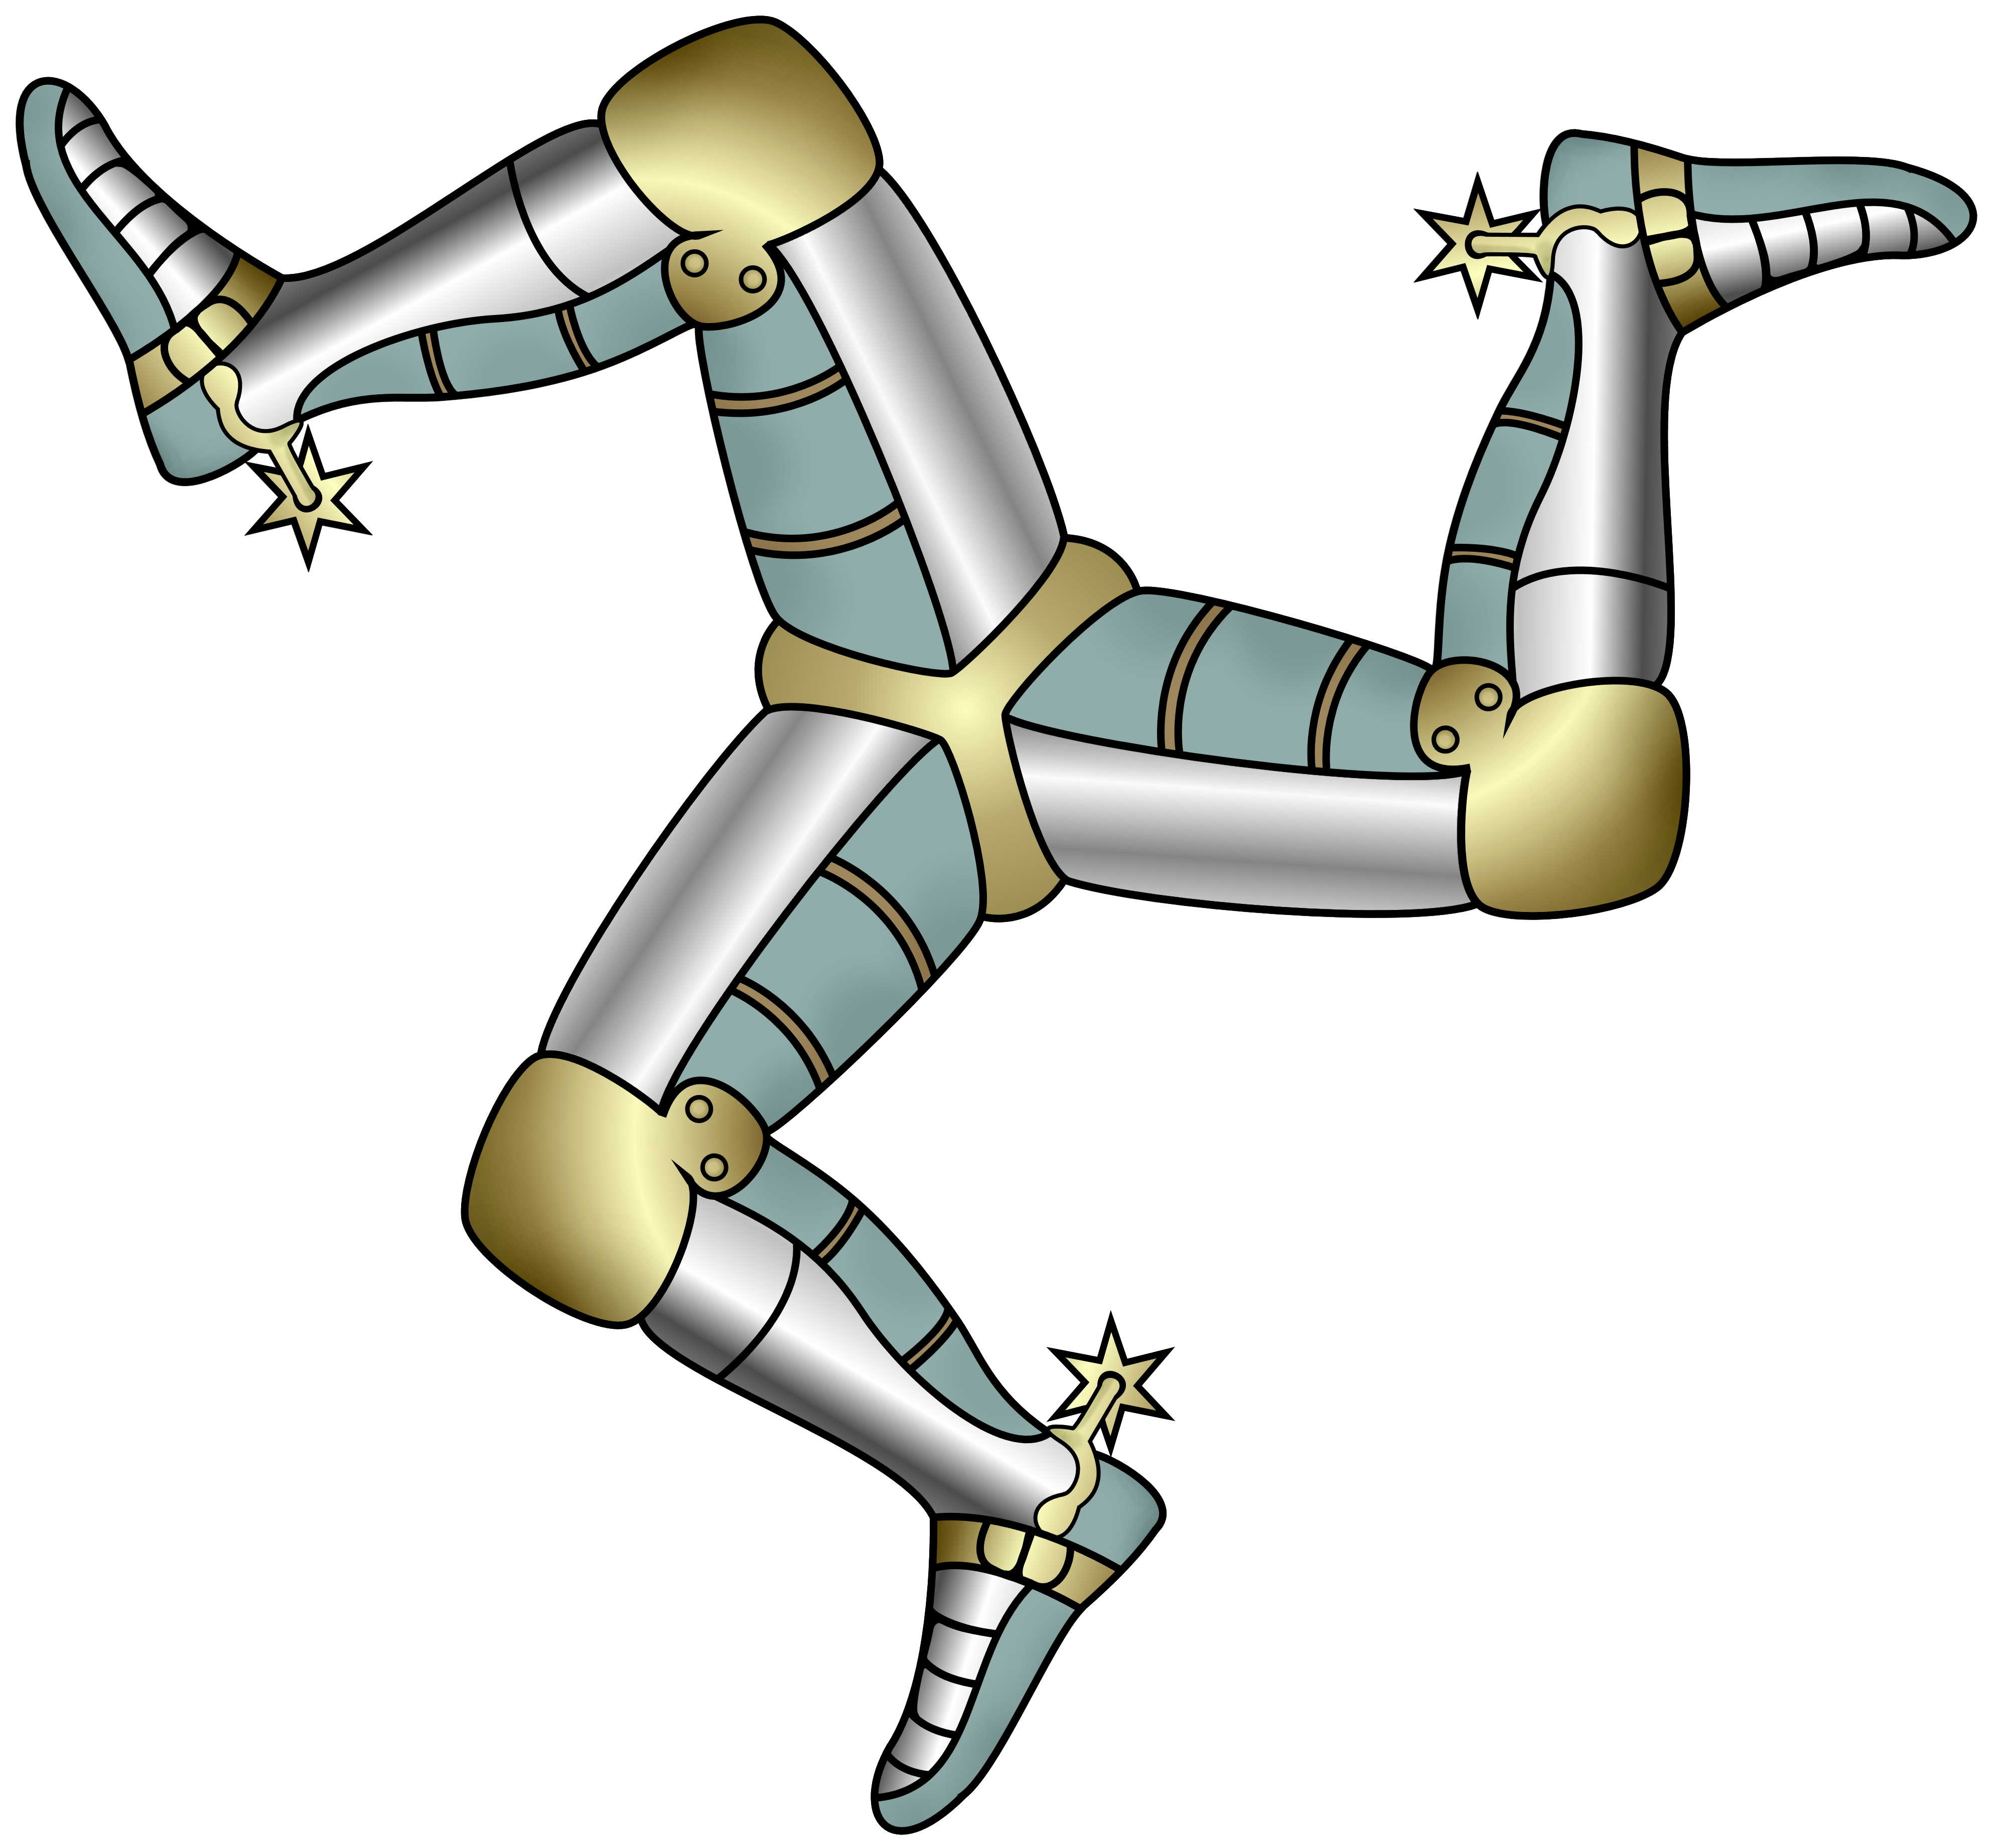
\includegraphics[width=1.5in]{Triskelion.jpg}\\[3pt]%
The three legs of Man.\end{center}}
\end{example}

\begin{example}This is illustrated in the figure to the right.\marginnote{\vspace{-2.2in}\begin{center}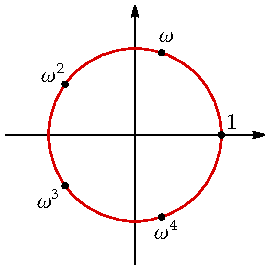
\includegraphics{FifthRootsOfUnity}\end{center}\vspace{-0.15in}The number $\beta=\omega^3$ is a primitive fifth root of unity.}
\end{example}

\end{document}
